\documentclass[tikz,border=5pt]{standalone}
\newcommand{\N}{50}
\newcommand{\NC}{10}
\pgfmathsetseed{233333}
\definecolor{c1}{RGB}{31,119,180}
\definecolor{c2}{RGB}{255,127,14}
\definecolor{c3}{RGB}{44,160,44}
\definecolor{c4}{RGB}{214,39,40}
\definecolor{c5}{RGB}{148,103,189}
\definecolor{c6}{RGB}{140,86,75}
\definecolor{c7}{RGB}{227,119,194}
\definecolor{c8}{RGB}{127,127,127}
\definecolor{c9}{RGB}{188,189,34}
\definecolor{c10}{RGB}{23,190,207}
\begin{document}
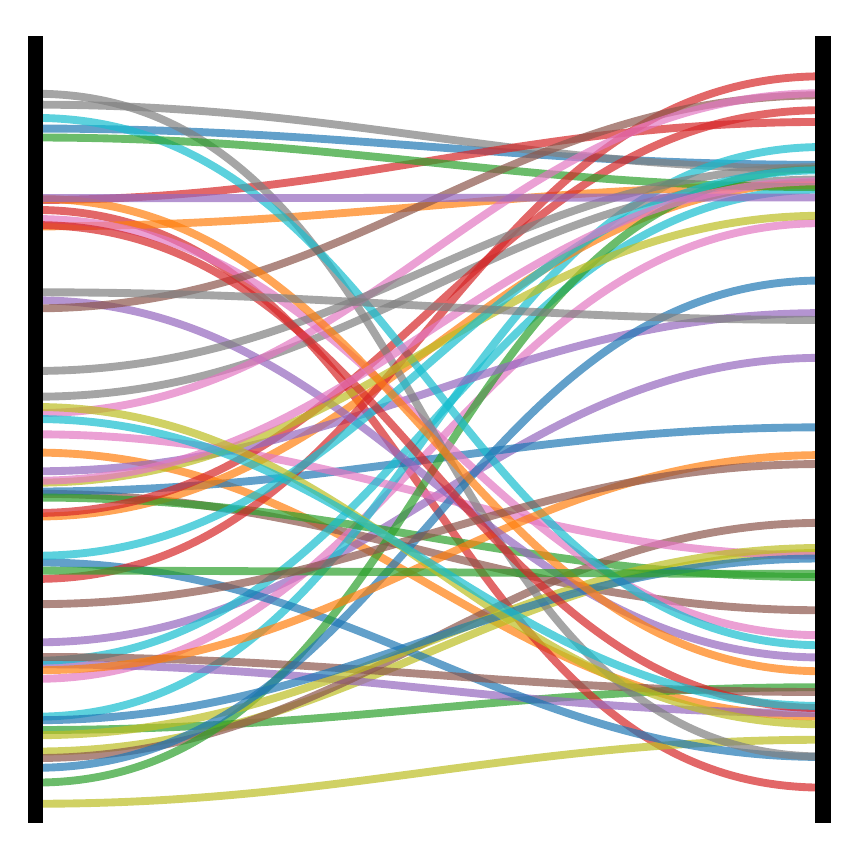
\begin{tikzpicture}
    \foreach \i in {1,...,\N} {
        \pgfmathtruncatemacro{\ci}{mod(\i-1,\NC)+1}
        \pgfmathsetmacro{\yA}{-4.8+9.6*rnd}
        \pgfmathsetmacro{\yB}{-4.8+9.6*rnd}
        \coordinate (A) at (-5,\yA);
        \coordinate (B) at (5,\yB);
        \draw[line width=1mm,c\ci,opacity=0.7] (A) to[out=0,in=180] (B);
        \fill[c\ci] (A) circle (1.2pt) (B) circle (1.2pt);
    }
    \draw[line width=2mm] (-5,-5) -- (-5,5) (5,-5) -- (5,5);
\end{tikzpicture}
\end{document}